\section{Results and Discussion}

% Wide figures are declared before the running text so the compositor can fill each page.

\begin{figure*}[!tbp]
\begin{minipage}{\textwidth}
\centering
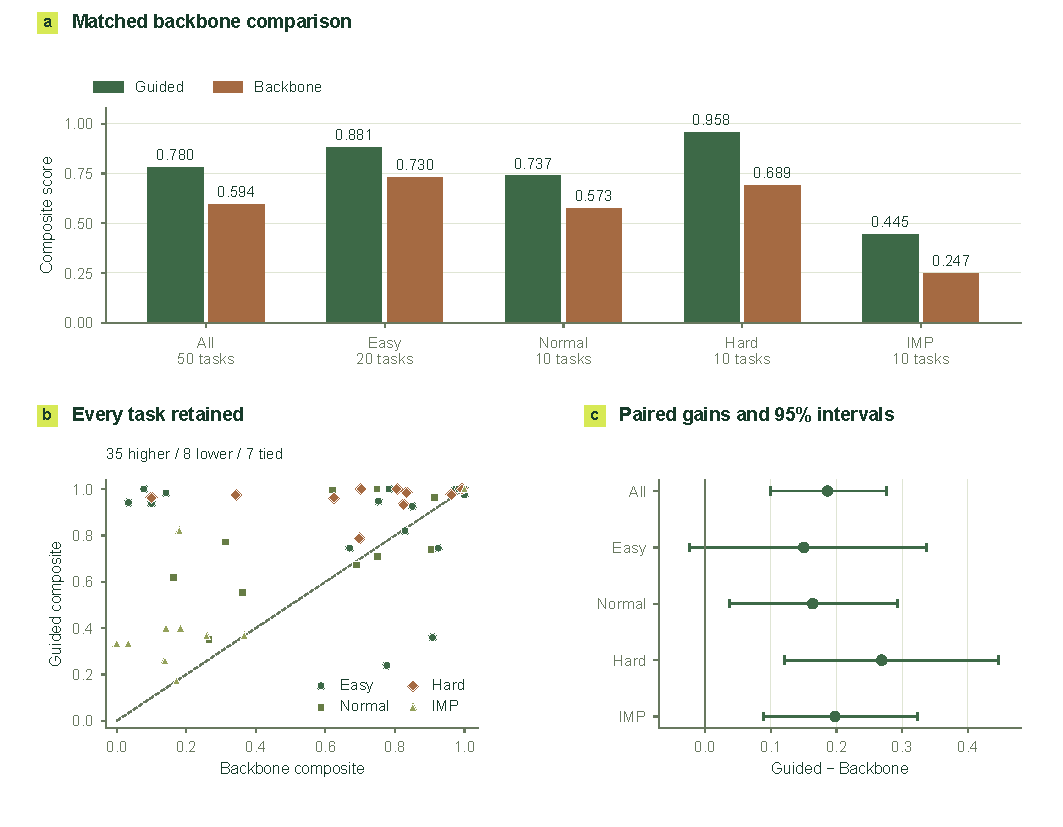
\includegraphics[width=\textwidth]{figures/bench_overview.pdf}
\caption{P2 benchmark outcomes under the archive-adjudicated track. (a) Guided and the same-backbone Standard baseline across all 50 tasks and each tier. (b) All 50 paired task outcomes. (c) Mean paired score differences with 95\% percentile intervals from 100,000 task-level bootstrap resamples. Each task has one run per configuration; Easy contains 20 tasks and the other tiers contain 10 each.}
\label{fig:bench-overview}
\end{minipage}
\end{figure*}

\begin{figure*}[!tbp]
\begin{minipage}{\textwidth}
\centering
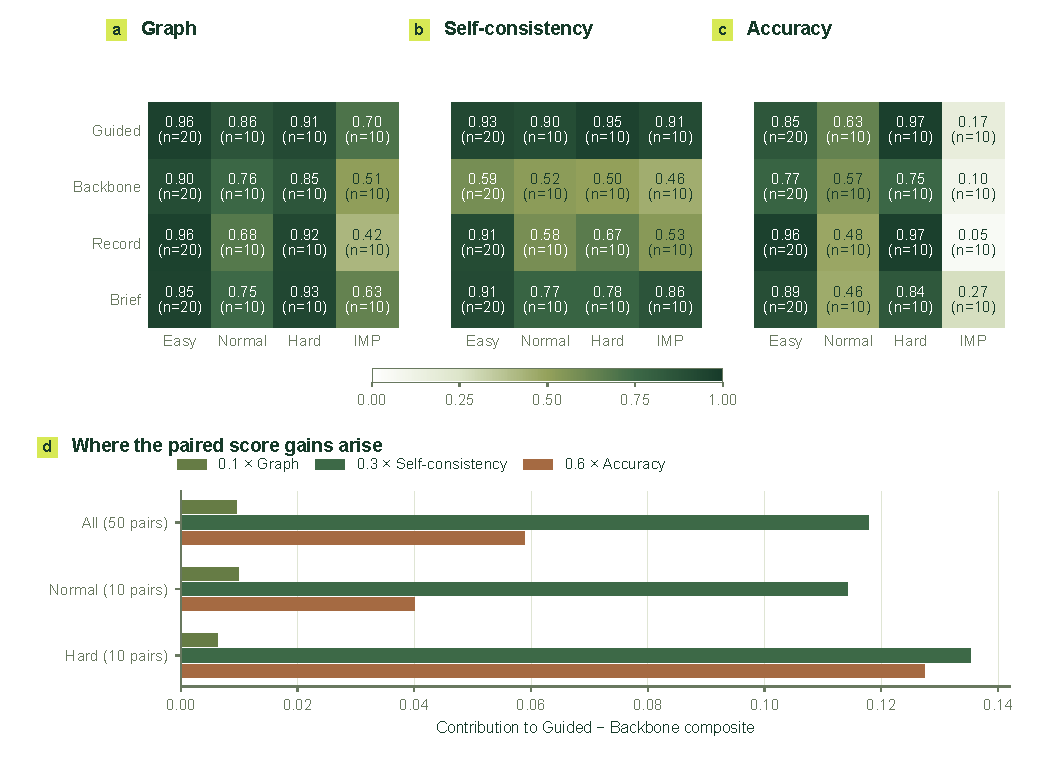
\includegraphics[width=\textwidth]{figures/bench_components.pdf}
\caption{CloudraBench score layers across all 200 organized runs. (a--c) Means of Graph, Self-consistency, and Accuracy in each arm and tier, using 50 tasks per arm overall, 20 Easy tasks, and ten tasks in each other tier. (d) Guided--Backbone mean differences decomposed with the fixed weights 0.1/0.3/0.6, using all 50 pairs, ten Normal pairs, and ten Hard pairs. Components are aligned with the final organized totals using each run's recorded research materials and score records.}
\label{fig:bench-components}
\end{minipage}
\end{figure*}

\begin{figure*}[!tbp]
\begin{minipage}{\textwidth}
\centering
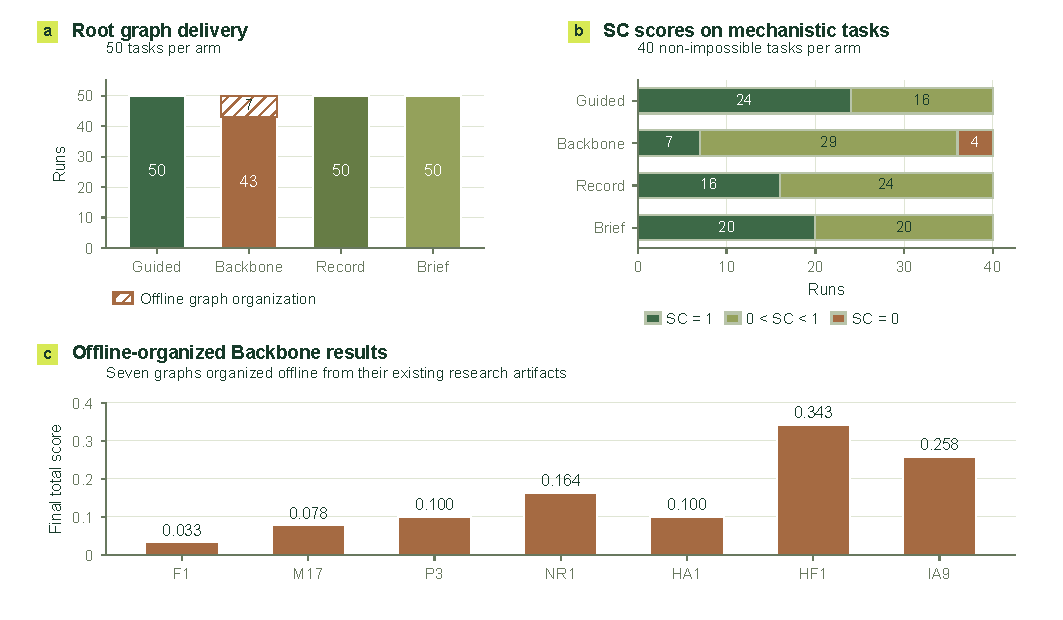
\includegraphics[width=\textwidth]{figures/bench_delivery.pdf}
\caption{Runtime graph delivery and final scientific support in P2. (a) Original root mechanism graphs across 50 tasks per arm: Guided 50, Backbone 43, Record 50, and Brief 50. The hatched segment marks seven additional Backbone graphs assembled offline from the runs' own research materials; the organized set contains 50 graphs per arm. (b) Final continuous self-consistency (SC) scores for all 40 non-Impossible tasks per arm, separating SC = 1, partial positive credit, and SC = 0. Full-score counts are 24, 7, 16, and 20; Backbone has four zero-score tasks. (c) Organized composite scores for the seven Backbone tasks without runtime root graphs, ranging from 0.0333 to 0.3425 (mean 0.1537).}
\label{fig:bench-delivery}
\end{minipage}
\end{figure*}

\begin{figure*}[!tbp]
\begin{minipage}{\textwidth}
\centering
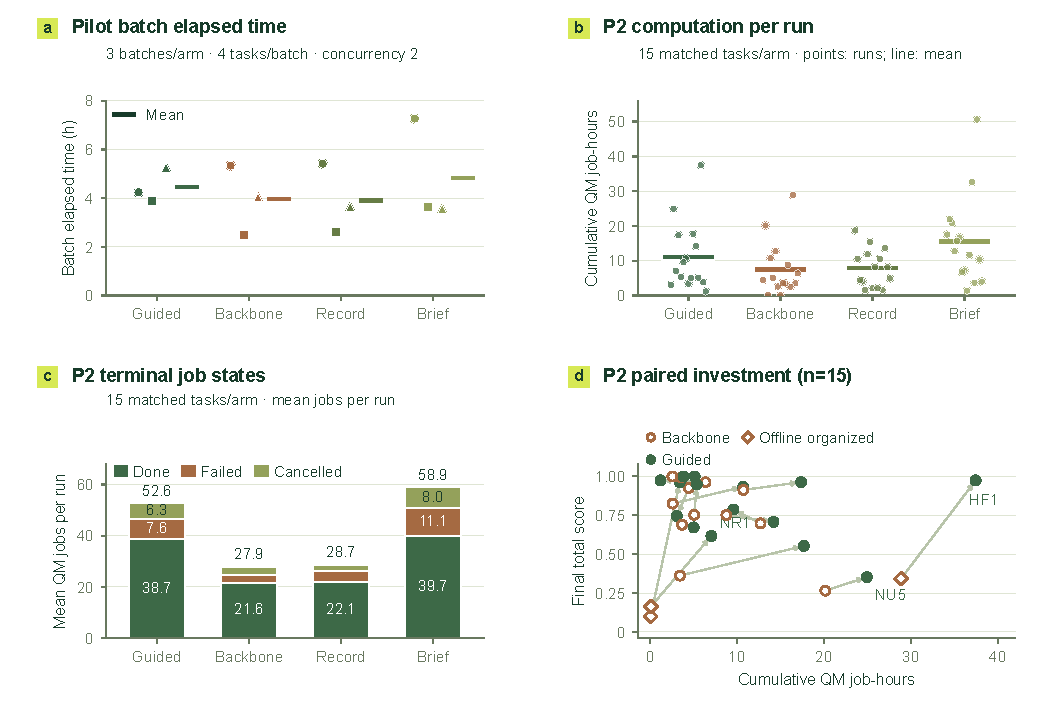
\includegraphics[width=\textwidth]{figures/bench_speed.pdf}
\caption{Research elapsed time and computational investment. (a) Twelve P1b four-task batches at concurrency two, three per arm; lines mark means. (b) Cumulative QM process durations for the 15 P2 tasks shared by all arms. (c) Mean completed, failed, and cancelled jobs in that cohort. (d) Same-task Backbone-to-Guided changes in investment and final score; diamonds mark offline-organized Backbone graphs. Job-hours sum process walltime; panel a measures batch latency. Backbone/M1 effort is reconstructed from native CPU time divided by four.}
\label{fig:bench-speed}
\end{minipage}
\end{figure*}

\begin{figure*}[p]
\begin{minipage}{\textwidth}
\centering
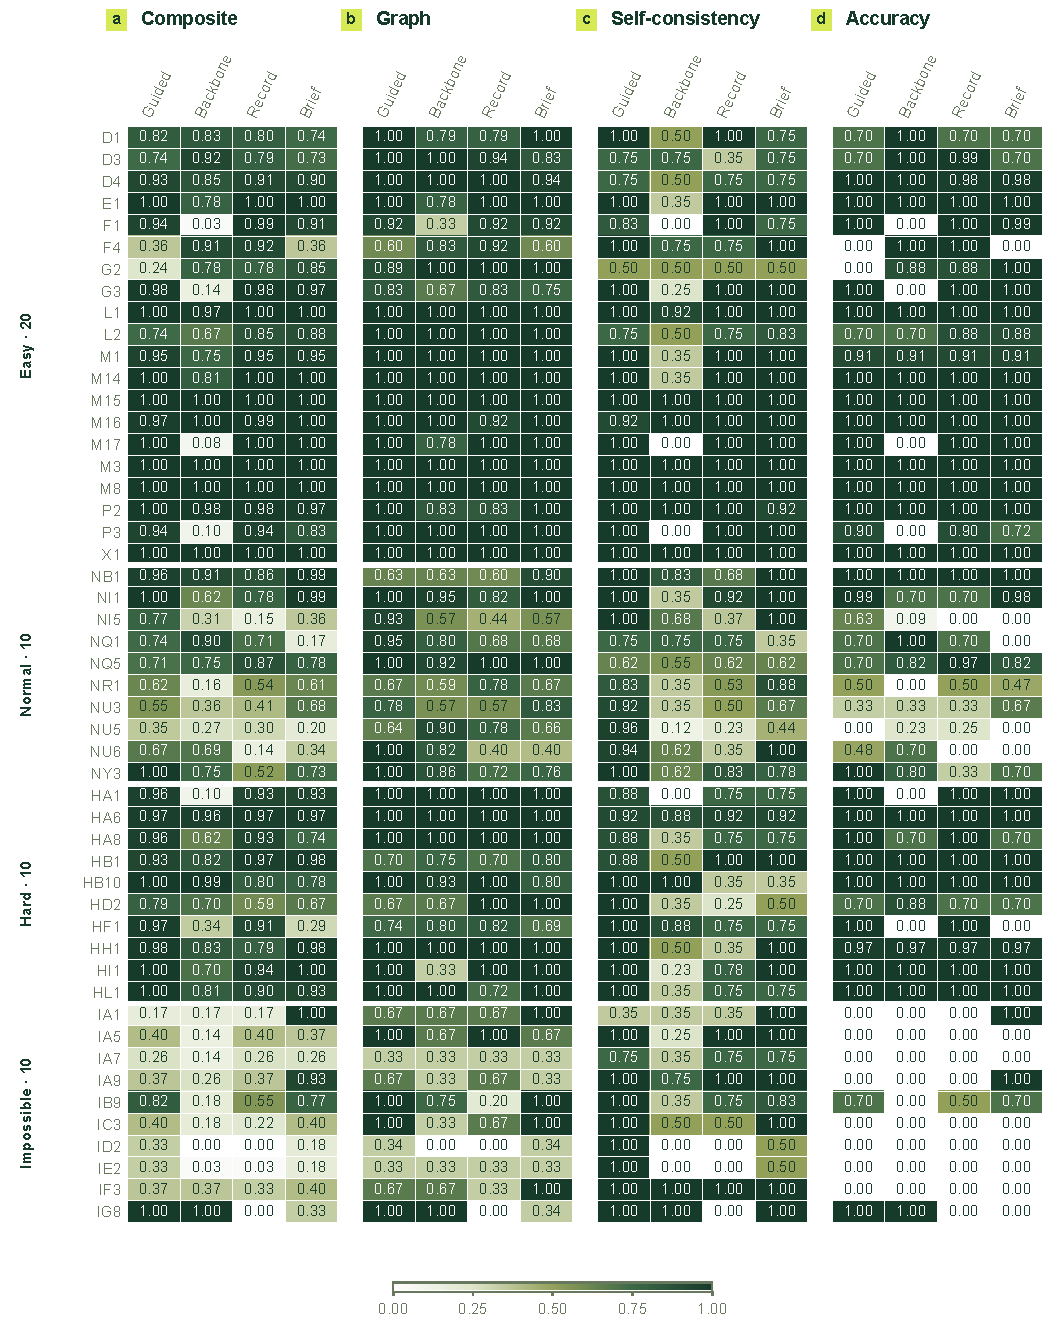
\includegraphics[width=\textwidth]{figures/bench_tasks_all.pdf}
\caption{Complete CloudraBench results for all 50 tasks and four configurations. The aligned blocks show composite, Graph, Self-consistency, and Accuracy on the same 0--1 scale; all 800 cells are present. Values are rounded to two decimals; the source table retains full precision.}
\label{fig:bench-tasks}
\vspace{6pt}
\end{minipage}
\end{figure*}

\begin{figure*}[!tbp]
\begin{minipage}{\textwidth}
\centering
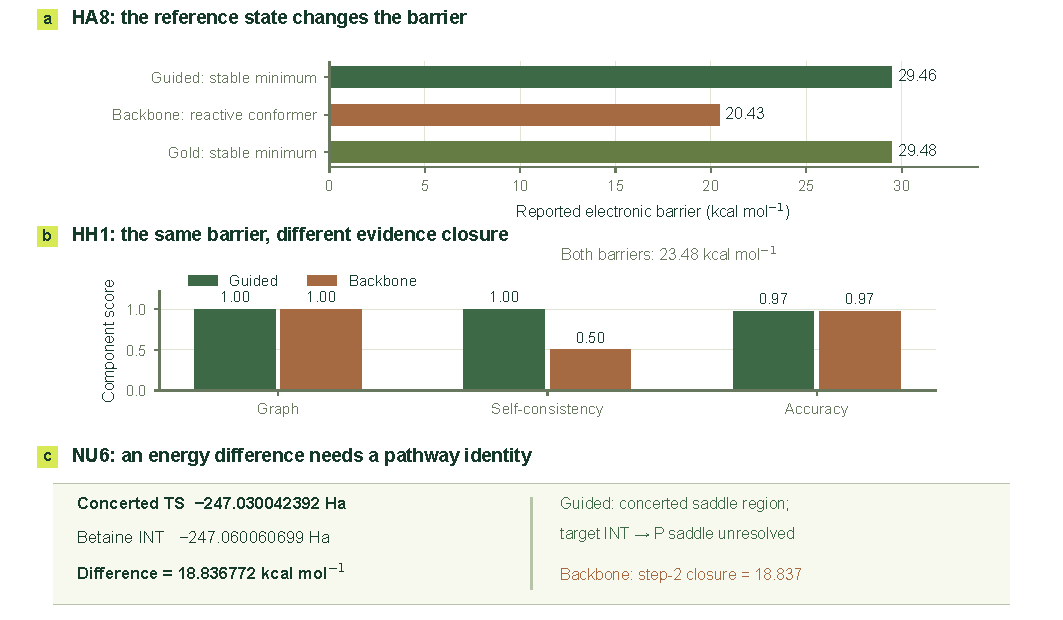
\includegraphics[width=\textwidth]{figures/bench_cases.pdf}
\caption{Scientific attribution in matched Guided--Backbone tasks. (a) HA8 barriers use stable-minimum or reactive-conformer references. (b) HH1 retains the same barrier and accuracy, with different evidence closure. (c) NU6's recorded energy difference is assigned to different pathways. Values and assignments derive from the archived records.}
\label{fig:bench-cases}
\end{minipage}
\end{figure*}

\begin{figure*}[!tbp]
\begin{minipage}{\textwidth}
\centering
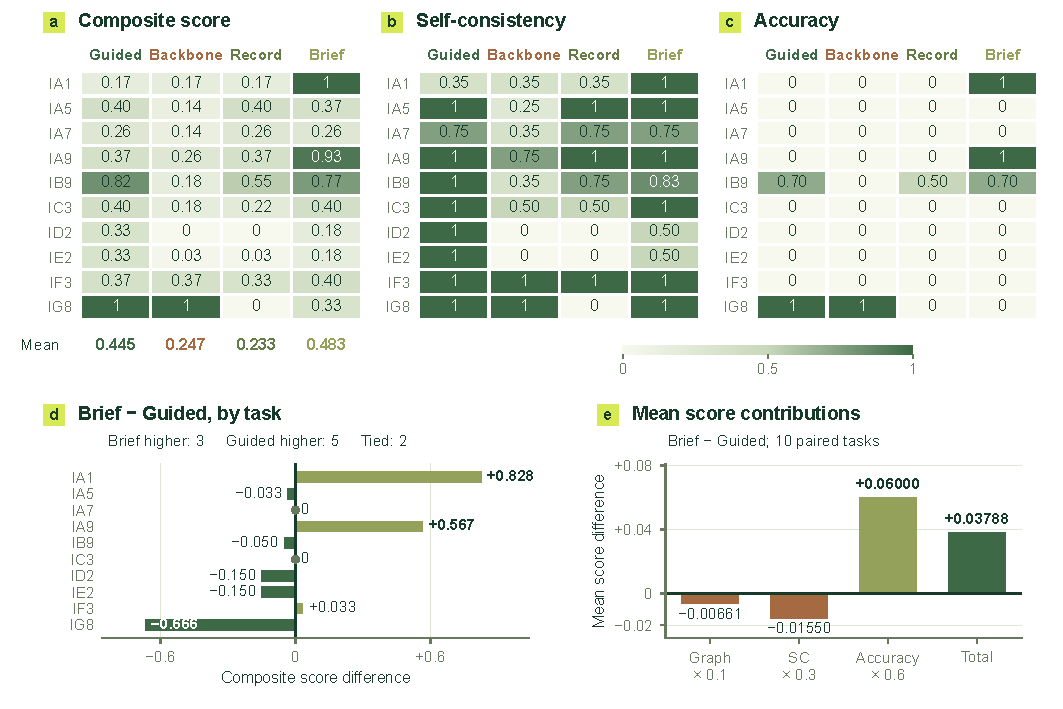
\includegraphics[width=\textwidth]{figures/bench_imp.pdf}
\caption{Impossible-tier outcomes and the brief-diagnostic ablation. (a--c) Composite, self-consistency (SC), and accuracy for all ten tasks and four arms, using the complete organized scores on a common 0--1 scale. Backbone denotes the actual same-backbone Standard arm. (d) Paired Brief-minus-Guided differences: the mean advantage of 0.03788 is concentrated in IA1 and IA9, with an opposite outcome in IG8; Guided scores higher on five tasks, Brief on three, and two tie. (e) The mean difference decomposes into weighted accuracy (+0.06000), Graph ($-0.00661$), and SC ($-0.01550$); the small discrepancy in their sum reflects rounding of saved totals. The paired task-bootstrap 95\% interval is $-0.188$ to +0.284; task-specific claims are analyzed below.}
\label{fig:bench-imp}
\end{minipage}
\end{figure*}

\begin{figure*}[!tbp]
\begin{minipage}{\textwidth}

\centering
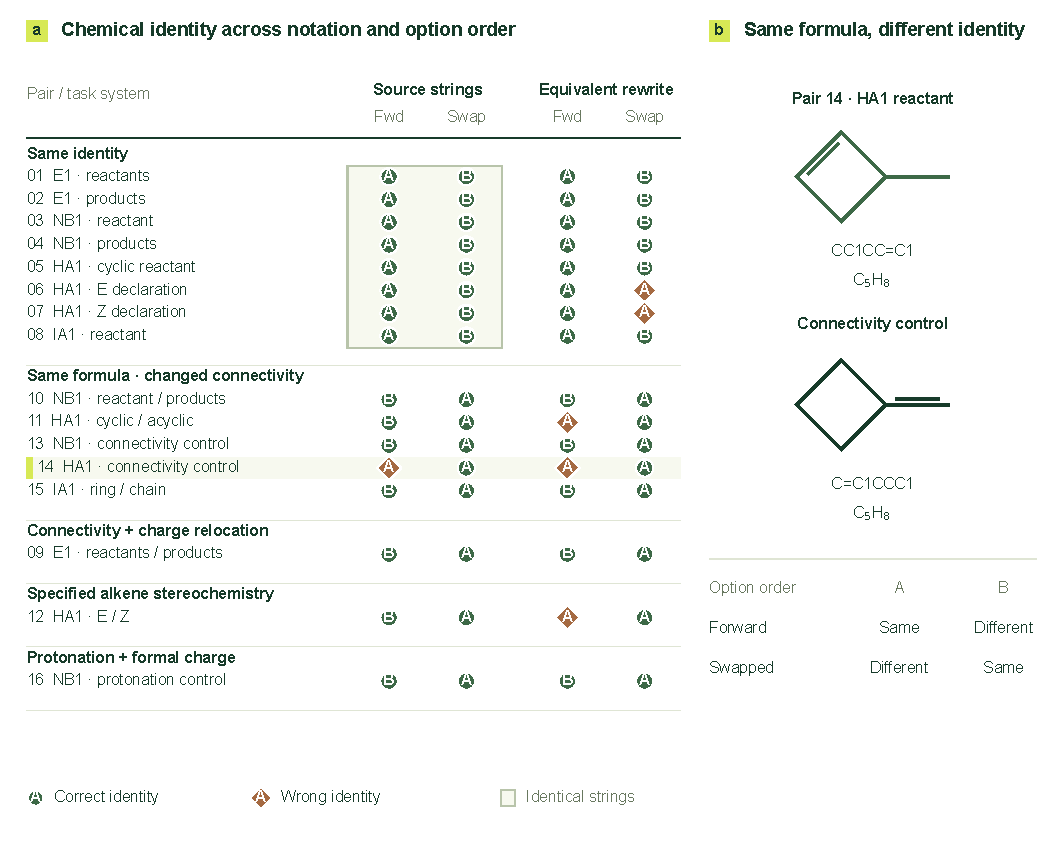
\includegraphics[width=\textwidth]{figures/fig06.pdf}
\caption{Molecular-identity judgments under changes in molecular representation and option order. Each of the 16 molecular pairs has four input conditions. Circles and diamonds indicate correct and incorrect judgments, respectively; the letters retain the model's actual answers. Shaded regions denote identical-string conditions. The right panel shows the pair-14 connectivities \texttt{CC1CC=C1} and \texttt{C=C1CCC1}, both C\textsubscript{5}H\textsubscript{8}, and the meanings of the answer options.}
\label{fig:06}
\end{minipage}
\end{figure*}

\begin{figure*}[!tbp]
\begin{minipage}{\textwidth}
\begin{minipage}[t]{.65\textwidth}
\vspace{0pt}
\centering
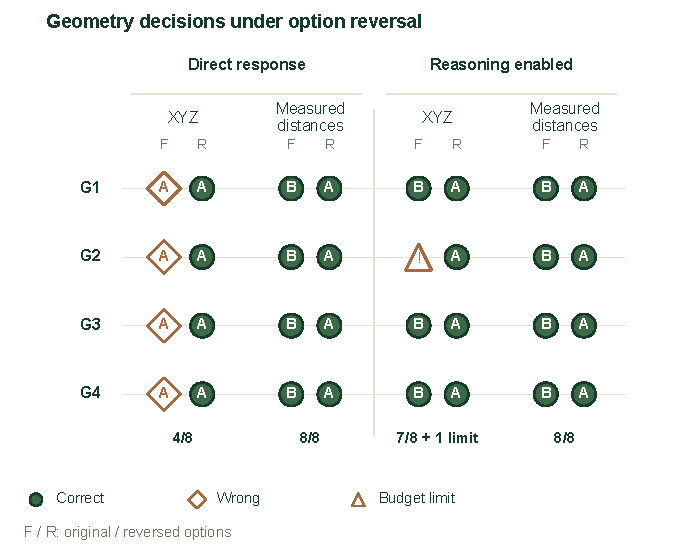
\includegraphics[width=\linewidth]{figures/fig07.pdf}
\caption{Geometry judgments under coordinate inputs and measured-distance inputs. Four source structures are compared under direct response and reasoning-enabled conditions, each with original (F) and reversed (R) option order. Circles indicate correct judgments, diamonds incorrect judgments, and the triangle a response that reached the output budget. Letters retain the actual answers.}
\label{fig:07}
\end{minipage}\hfill
\begin{minipage}[t]{.31\textwidth}
\vspace{0pt}
\centering
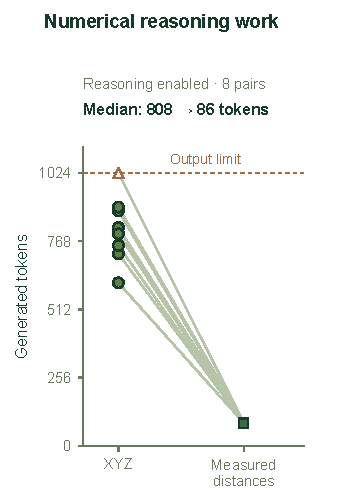
\includegraphics[width=\linewidth]{figures/fig08.pdf}
\caption{Generated-token counts with reasoning enabled. Each line connects Cartesian-coordinate input and measured-distance input for the same source structure and option order; eight paired comparisons are shown. The dashed line marks the output limit.}
\label{fig:08}
\end{minipage}
\end{minipage}
\end{figure*}

\begin{figure*}[!tbp]
\begin{minipage}{\textwidth}
\centering
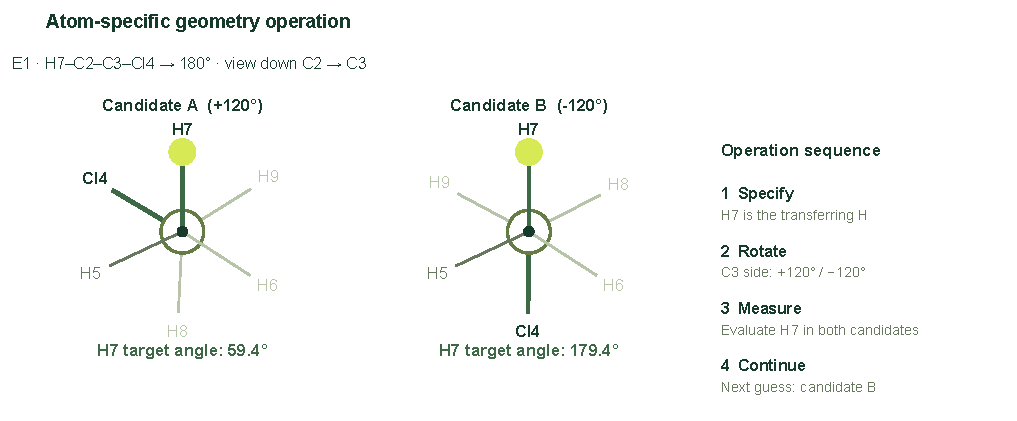
\includegraphics[width=.92\textwidth]{figures/fig09.pdf}
\caption{Target-specific geometry operations in E1. Newman projections retain the directions of the original candidate coordinates viewed down C2\(\to\)C3. H7 is the specified transferring atom. Candidate A and candidate B give target angles of 59.4° and 179.4°, respectively. The operation sequence is shown alongside the projections.}
\label{fig:09}
\vspace{5pt}
\begin{minipage}[t]{.48\textwidth}
\vspace{0pt}
\centering
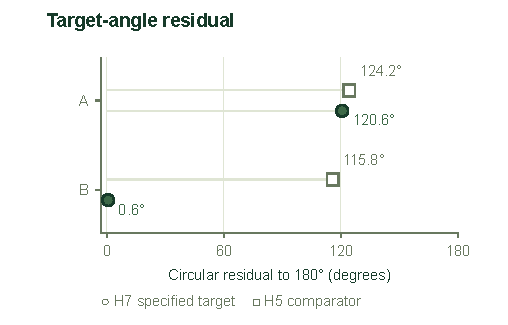
\includegraphics[width=\linewidth]{figures/fig10.pdf}
\caption{Circular angular residuals from the specified 180° target for candidates A and B. H7 is the specified target atom; H5 is the comparator.}
\label{fig:10}
\end{minipage}\hfill
\begin{minipage}[t]{.48\textwidth}
\vspace{0pt}
\centering
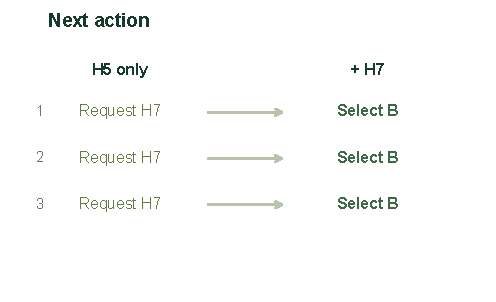
\includegraphics[width=\linewidth]{figures/fig11.pdf}
\caption{Next-action choices under three local option permutations. When only H5 measurements are supplied, the model requests H7 measurements; with H7 supplied, it selects candidate B.}
\label{fig:11}
\end{minipage}
\end{minipage}
\end{figure*}

\begin{figure*}[!tbp]
\begin{minipage}{\textwidth}
\centering
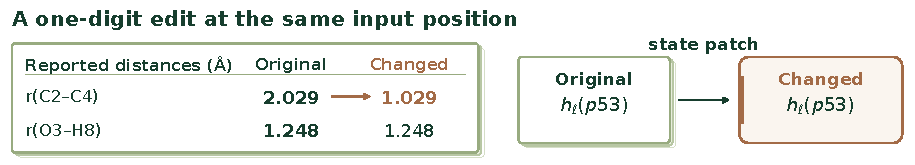
\includegraphics[width=.92\textwidth]{figures/fig12.pdf}
\caption{Intervention on a single reported distance. A one-digit edit changes the C2–C4 distance from 2.029 to 1.029 Å while O3–H8 remains 1.248 Å. The original-input residual state at token position 53 is inserted into the changed-input run at a specified layer. Token positions are zero-based.}
\label{fig:12}
\vspace{4pt}
\centering
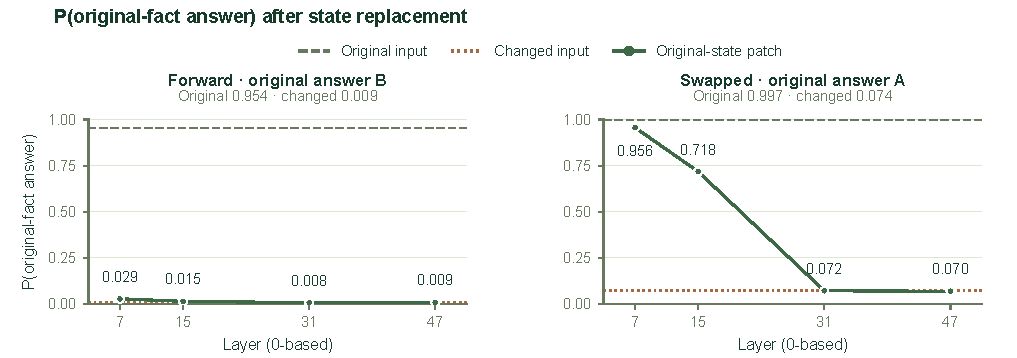
\includegraphics[width=.92\textwidth]{figures/fig13.pdf}
\caption{Original-fact answer probability after state replacement. Curves show full-vocabulary probability mass for the original-fact answer under forward (B) and swapped (A) option order, including bare and leading-space token spellings. Horizontal lines show original-input and changed-input baselines. Layer indices are zero-based.}
\label{fig:13}
\vspace{4pt}
\centering

\includegraphics[width=.92\textwidth]{figures/fig14.pdf}
\caption{Control substitutions for the state-intervention experiment. Same-state self replacement at p53 and replacement of the unchanged prefix at p0 preserve all vocabulary logits in both option orders. The table reports the maximum absolute logit difference. Token positions are zero-based.}
\label{fig:14}
\end{minipage}
\end{figure*}

\begin{figure*}[!tbp]
\begin{minipage}{\textwidth}

\begin{minipage}[t]{.48\textwidth}
\vspace{0pt}
\centering
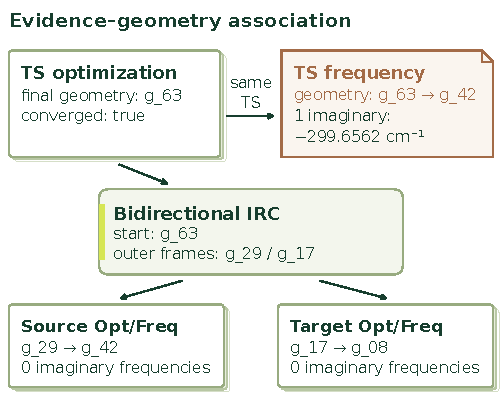
\includegraphics[width=\linewidth]{figures/fig15.pdf}
\caption{Evidence--geometry association in E1. The frequency geometry reference changes from g\_63 to g\_42 while local termination, convergence, energy, and frequency values remain fixed. Arrows retain the TS--IRC--endpoint optimization/frequency chain.}
\label{fig:15}
\end{minipage}\hfill
\begin{minipage}[t]{.48\textwidth}
\vspace{0pt}
\centering
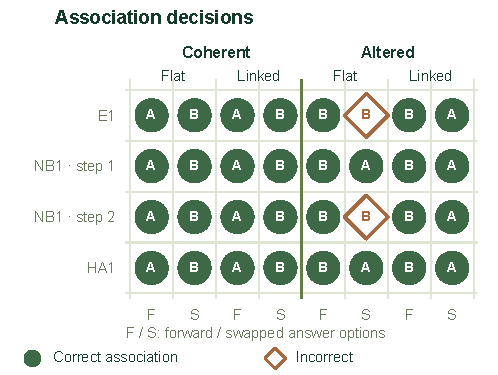
\includegraphics[width=\linewidth]{figures/fig16.pdf}
\caption{The 32 association judgments cross four source chains, coherent/altered links, flat/linked presentation, and forward/swapped answer order. Saved A/B responses and correctness markers are retained.}
\label{fig:16}
\end{minipage}
\end{minipage}
\end{figure*}

\begin{figure*}[!tbp]
\begin{minipage}{\textwidth}
\centering
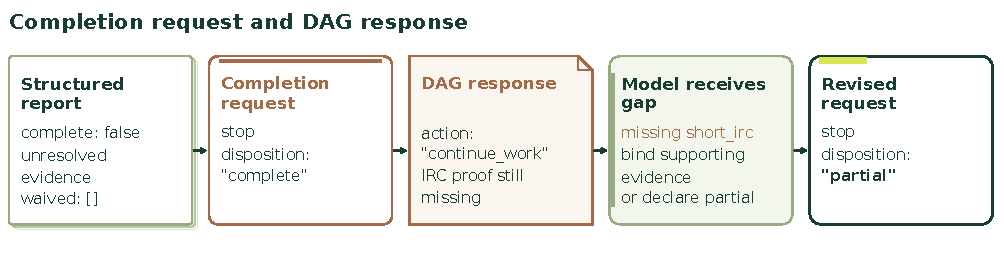
\includegraphics[width=.96\textwidth]{figures/fig17.pdf}
\caption{Completion requests and DAG feedback in the original IA1 trajectory. A report with unresolved evidence is followed by a completion request, a response identifying missing short\_irc proof, feedback to the model, and a revised partial-completion request.}
\label{fig:17}
\end{minipage}
\end{figure*}




















\subsection{End-to-end benchmark evaluation}

We first report the final organized composite scores and then examine their graph, self-consistency, and accuracy components. Offline organization assembles the mechanism graph from each run's own research materials and aligns its existing score records. The resulting 200-run table contains all three components for every run, with an overall composite mean of 0.7051. Figures~\ref{fig:bench-overview}--\ref{fig:bench-tasks} distinguish final delivery, the support established for individual calculations, and agreement with the task's answer.

\subsubsection{Cloudra improves research delivery relative to the same backbone}

Guided obtained a mean composite score of 0.7803, compared with 0.5940 for Standard. Across the 50 task pairs, the mean improvement was 0.1863, with a 95\% task-bootstrap interval of [0.1003, 0.2759]. Guided scored higher on 35 tasks, lower on eight, and equally on seven; the median paired difference was 0.1080 (Figure~\ref{fig:bench-overview}). The improvement therefore appears across many research questions rather than arising solely from a small increase in the highest-scoring runs.



Guided's mean over its ten lowest-scoring tasks was 0.3181, compared with 0.0930 for Standard.



The most consistent difference occurred in the Hard stereochemistry tasks. Guided averaged 0.9577 and Standard 0.6888, a paired increase of 0.2689 [0.1213, 0.4459], with Guided scoring higher on all ten tasks. These tasks require the system to maintain the identity of competing configurations or channels, compare the relevant barriers, and attach evidence to the corresponding conclusion. The observed improvement thus concerns the completion of a comparative chemical study, including the organization of the evidence supporting its stereochemical outcome.

On Normal tasks, Guided averaged 0.7370 versus 0.5731, an increase of 0.1640 [0.0365, 0.2922], with seven wins and three losses. Easy-task means were 0.8809 and 0.7305, respectively; the paired median difference was 0.0209, showing a different pattern from the broadly positive Hard comparison. Impossible-task means were 0.4451 and 0.2473. Their interpretation depends on whether the run addressed the requested method-limited negative target, so these tasks are examined separately below.





\subsubsection{Evidence closure accounts for much of the component-level gain}

Separating the three score components locates where the workflows diverged (Figure~\ref{fig:bench-components}). Graph measures the delivered coverage and identities of the requested species and steps. Self-consistency measures the support linking saddle points, frequencies, IRC starts, and endpoint optimization/frequency calculations. Accuracy measures agreement with the task's numerical or negative target. A run can therefore give a close numerical answer while leaving its supporting path incomplete, or establish a coherent local calculation that does not answer the requested research question.

Across all 50 Guided--Standard task pairs, the weighted graph contribution to the mean improvement was +0.0095, self-consistency contributed +0.1179, and accuracy +0.0589, accounting together for the composite gain of 0.1863. For the 20 Normal and Hard tasks, the mean gain was 0.2164, with contributions of +0.0080 from graph, +0.1247 from self-consistency, and +0.0837 from accuracy. Within the ten Normal tasks, the corresponding contributions were +0.0098, +0.1141, and +0.0400; within the ten Hard tasks they were +0.0063, +0.1353, and +0.1274.



The full-task decomposition therefore locates gains in both scientific evidence closure and the requested answers. On Hard tasks, the accuracy improvement is comparable in size to the self-consistency improvement.



HH1 provides a direct example. Guided and Standard both reported a binaphthyl racemization barrier of 23.48 kcal/mol, close to the 23.01 kcal/mol reference. Both had graph scores of 1 and accuracy scores of approximately 0.973. Their self-consistency scores were 1.0 and 0.5, producing composite scores of 0.9838 and 0.8338, respectively. The archived Standard study contained candidate channels and IRC inputs, but its accepted evidence did not complete the required endpoint connections. Guided attached the path evidence to the corresponding saddle and endpoints. HI1 shows a related pattern: accuracy was approximately 1 in both runs, while self-consistency increased from 0.2333 to 1.0 and the composite score from 0.7032 to 0.9999. These comparisons identify an added layer of research completion after a promising numerical answer has already been obtained.





\subsubsection{Delivery artifacts and graded scientific support remain distinct}

The root delivery graph and the evidence carried by that graph describe different parts of the research process (Figure~\ref{fig:bench-delivery}). During the original runs, Standard delivered root graphs for 43 of 50 tasks, while Guided, Record, and Brief-errors each delivered 50. The seven Standard tasks without runtime root graphs were F1, HA1, HF1, IA9, M17, NR1, and P3. Offline organization assembled their graphs from the corresponding runs' existing materials, producing a complete 50-task set for every configuration.

The seven Standard studies averaged 0.1537 after organization, compared with 0.8285 for Guided on the same tasks, and contributed 50.7\% of the total Guided--Standard difference. Their individual scores ranged from 0.0333 to 0.3425. The contrast connects the runtime completion decision to the amount of research ultimately available for delivery: computations and candidate descriptions could remain in a run's records while the requested pathway or comparative conclusion had not yet been completed. The organized graph preserves that research state for evaluation.



The graded self-consistency distribution reveals a further difference among the completed task records. For the 40 non-Impossible tasks in each configuration, Guided had self-consistency exactly equal to 1 on 24 tasks and partial positive credit on 16. Standard had seven full-score, 29 partial-score, and four zero-score tasks. Record had 16 full-score and 24 partial-score tasks; Brief-errors had 20 of each. Figure~\ref{fig:bench-delivery} presents these complete evidence-score distributions alongside the separate runtime graph-delivery counts. This view preserves the amount of scientific support assembled within each study.

\subsubsection{Ablations separate available capabilities from persistent guidance}

Record averaged 0.7044 and Brief-errors 0.7415 across all 50 tasks. Guided exceeded Record by 0.0759 [0.0121, 0.1438], with 27 wins, eight losses, and 15 ties. On all 20 Normal and Hard tasks together, the mean Guided--Record difference was 0.1468: graph contributed +0.0083, self-consistency +0.0919, and accuracy +0.0466. Keeping the tools and a place to record results therefore produced a different outcome from keeping unresolved scientific requirements active throughout the study.





\subsubsection{Elapsed research time and computational effort describe different gains}

Figure~\ref{fig:bench-speed} presents the timing information from the repeated-task study alongside the computational effort available for P2. For the repeated study, the measurement unit is a complete four-task batch at a concurrency of two, with three observed batches per configuration. Mean batch elapsed times were 4.451, 3.958, 3.894, and 4.827 hours for Guided, Standard, Record, and Brief-errors, respectively. Guided batches took 12.5\% longer than Standard and 7.8\% less time than Brief-errors on average. The figure shows all 12 observed batches, retaining their variation and original outcomes. These measurements include the batch's research lifecycle, waiting for calculations, and continuation after results return.

P2 effort is summarized over the 15 deeply inspected tasks shared by all four configurations. Guided used 11.08 job-hours per task, Standard 7.55, Record 7.88, and Brief-errors 15.59. The corresponding final composite means were 0.8124, 0.6495, 0.7360, and 0.7273. Guided used 46.7\% more cumulative job time than Standard while increasing the mean score by 0.1629; relative to Brief-errors, it used 28.9\% less job time and scored 0.0851 higher. Guided was both faster in cumulative job time and higher-scoring than Brief-errors on seven of the 15 paired tasks.



The job counts add information about the character of this expenditure.



Across the common tasks, Guided submitted 789 recorded quantum-chemical jobs, Standard 419, Record 431, and Brief-errors 883. Recorded failed-job counts were 114, 45, 62, and 167, respectively, with cancellations recorded separately. The four difficult studies NU3, NU5, NU6, and NR1 accounted for 163.5 job-hours across their 16 runs, 24.3\% of the 673.82 job-hours in the available 63-run effort archive. These data locate a substantial part of computational expenditure in studies where additional attempts did not uniformly complete the missing network. In the archived Standard missing-graph cases, calculations could also outlive the research session, leaving subsequent results outside an active study. Continuing the research after a calculation returns is therefore part of the delivered workflow measured here.

Guided exceeded Brief-errors by 0.0388 overall, with an interval of [$-0.0317$, 0.1076], 26 wins, ten losses, and 14 ties. The comparison varied by research demand: Guided's mean advantage was 0.1514 on Normal and 0.1295 on Hard, whereas Brief-errors had the higher Impossible mean. Together with the common-task effort comparison, these observations support examining what a diagnostic enables the system to repair: a specific saddle assignment, a path endpoint, an energy reference, or the judgment that the permitted method cannot support the requested claim. More diagnostic text does not impose the same ordering across these different decisions.









\subsubsection{Per-task patterns identify the chemical relations that need to persist}

Figure~\ref{fig:bench-tasks} places all 50 tasks and four configurations alongside their complete score components. The resulting landscape shows both consistent gains and specific reversals. Guided performed strongly across the Hard comparative studies, while NB1 and NI1 show that multistep studies could also retain high scores and strong evidence support. NB1 scored 0.9628 under Guided, 0.9128 under Standard, and 0.9900 under Brief-errors; Guided and Brief-errors both had self-consistency 1. NI1 scored 0.9958 under Guided and 0.6196 under Standard, with self-consistency 1 and 0.35. In contrast, NQ5 favored Record over Guided, and NU3 favored Brief-errors. These differences make the individual target steps and evidence relationships more informative than a single ordering by network length.

Three archived comparisons clarify which chemical relations matter (Figure~\ref{fig:bench-cases}). In HA8, Guided reported 29.46 kcal/mol and Standard 20.43 kcal/mol against a reference of 29.48 kcal/mol. The archive traces this 9.03 kcal/mol difference to the energy reference: the lowest all-s-trans reactant minimum in Guided and a reactive cisoid conformer in Standard. Local IRC connectivity and the stable-species reference for an activation energy consequently need to remain associated without being conflated.



The former identifies the structures reached by a particular path; the latter determines the energetic starting point specified by the research question.



NU6 exposes a related issue in path identity. Guided's recorded concerted saddle had an energy of $-247.030042392$ Ha and the betaine minimum $-247.060060699$ Ha, giving a difference of 18.836772 kcal/mol. Guided described this as an energy cost involving the concerted saddle region while retaining the target betaine-to-product ring-closure saddle as unresolved. Standard delivered 18.837 kcal/mol as the second-step ring-closure barrier. The numerical fingerprint thus locates the divergence in what scientific step an energy difference was taken to represent. Guided's attempts from interpolated betaine structures and constrained scan peaks repeatedly relaxed toward the direct reactant-to-product saddle region. The requested path identity had to be checked again after optimization, rather than being inherited from the name of its initial guess.

These cases complement the HH1 evidence comparison: the same research state must preserve which conformer defines the reference, which stationary point was actually found, which endpoints it connects, and which claim those results support. The Easy-tier comparisons resolve additional differences between the physical evidence and its reference matching or structured delivery. In F4, Guided scored 0.3601 and Standard 0.9083. Guided delivered a log-supported hydride-transfer barrier of 16.016 kcal/mol with graded self-consistency 1. Its accuracy of 0 arose from the historical reference encoding separated reactant fragments while the delivered pathway and reference barrier concerned the Lewis adduct.

In G2, Guided scored 0.2389 and Standard 0.7769. Guided's native logs supported an approximately 0.845-kcal/mol double-H-transfer barrier. After three rejections of numerical barrier declarations on a companion edge, the agent removed the numerical fields. Supervisor feedback prompted restoration, but a fourth rejection and a subsequent saddle-evidence check preceded their final removal, together with the saddle energy/log bindings. The final graph retained the values in text and received accuracy 0. Brief-errors retained the corresponding numerical result and scored 0.8500.

For Guided--Record, the F4 and G2 composite deficits were 0.5566 and 0.5380. Their sum, 1.0946, accounts for 86.3\% of the total Easy-tier net deficit of 1.2679. The accuracy values of 0.7 in D1, D3, and L2 followed the specified cap on numerical-deviation penalties. D1's barrier difference from Standard traced to the reactant-conformer reference; D3's mainly reflected different saddle energies. L2 distinguished reactive cZc and lower tZt references. Standard delivered both associated barriers, 18.99 and 28.28 kcal/mol, but reference matching selected the former. The Supplementary Information provides the workflow-level components, native evidence, and event chronology for these five tasks; all released scores are retained.





\subsubsection{Impossible tasks distinguish local support from the requested negative conclusion}

The Impossible tier tests whether research under xTB/PM7 reaches the specified method-limited conclusion. Brief-errors averaged 0.4829, Guided 0.4451, Standard 0.2473, and Record 0.2325 (Figure~\ref{fig:bench-imp}). Brief-errors exceeded Guided on three tasks and scored lower on five, with two ties. Its mean advantage of 0.0379 was concentrated in particular answers: IA1 contributed +0.8283 and IA9 +0.5666, whereas Guided's IG8 result contributed a difference of $-0.6661$ in the Brief-errors-minus-Guided direction.

In IA1, concerning cyclobutadiene's square-geometry automerization target, Brief-errors had graph, self-consistency, and accuracy scores of 1, while Guided's accuracy was 0. In IA9, concerning dioxetane thermolysis, Brief-errors and Guided both had self-consistency 1, but accuracy was 1 and 0, respectively. IG8 showed the opposite accuracy ordering for the chromium-dimer target. Across the seven tasks with the same accuracy score in Brief-errors and Guided, Brief-errors averaged 0.0500 lower. Its overall Impossible advantage decomposed into weighted contributions of $-0.0066$ from graph, $-0.0155$ from self-consistency, and +0.0600 from accuracy. The higher mean arose from the requested conclusions on specific tasks, while Guided retained stronger local support on several others.



Across all 40 Impossible runs, four had accuracy 1 and 14 combined self-consistency 1 with accuracy 0. This separation is visible directly in the component matrices. For example, both Guided and Brief-errors obtained self-consistency 1 in IA5, IC3, and IF3 without receiving accuracy credit for the requested negative target. Guided and Brief-errors both received partial accuracy of 0.7 in IB9, whose requested network contains positive and negative components. These outcomes retain the distinction between local computational support and the target claim.

The saved Brief-errors IC3 graph provides a concrete example of this distinction in scientific reporting. It marks the lowest open-shell singlet and its state-change edge inaccessible and withholds the requested singlet--triplet gap. The computed closed-shell singlet remains as a separate characterized branch, and the two method-dependent relative energies are explicitly excluded from the requested gap. The run therefore retained useful exploratory results while declining to promote them into an answer about a different electronic state. Its final accuracy score remained 0. The claim and its score are both retained here, with the score-mapping issue considered in the Discussion. This behavior complements the IA1, IA9, and IG8 score reversals by showing precisely which result was accepted as computable and which target claim remained unsupported.


















\subsection{From chemical intent to reliable geometric operations}


The following sections use archived research trajectories and Qwen3.8:27b local diagnostics to examine the interfaces implicated by these results: chemical identity, target-specific geometric operations, evidence associations, and the decision to end a study. The original trajectories locate concrete research problems; paired local inputs and internal-state interventions examine how particular information changes judgments and actions.

\subsubsection{Molecular identity provides a persistent reference for operations}



A geometric modification first requires identifying the molecule, atoms, and reaction center to which it applies. A molecule can be represented by different SMILES traversals, while a molecular formula can describe different connectivities. To examine how the model handles these distinctions, we constructed 16 molecular-identity pairs covering identical identities, connectivity changes within the same molecular formula, changes in connectivity and charge location, double-bond stereochemistry, and protonation changes. Each pair was presented using the original strings or equivalent rewritings and with two answer orders, yielding 64 judgments.



The model answered 58 correctly. Equivalent rewriting changed the semantic judgment in 4 of 32 matched representation comparisons; reversing answer order changed the judgment in 6 of 32 matched option-order comparisons. All six of the latter cases involved repeated selection of the letter A. One C\textsubscript{5}H\textsubscript{8} pair in Figure~\ref{fig:06} illustrates this behavior directly: an endocyclic and an exocyclic double bond define different connectivities, yet the model answered A under all four conditions, although A meant “same” in one order and “different” in the other. This result locates representation sensitivity in judgments about the chemical objects themselves and indicates the need for stable identity references throughout a research process.

Cloudra assigns this role to molecular topology, atom mapping, and reaction centers. These references allow subsequent measurements, fragment movements, and endpoint comparisons to remain attached to the originally specified objects as the model moves between descriptions and configurations. Atom correspondence also connects product-endpoint alignment, path interpolation, and reaction-center monitoring, allowing local geometric operations to proceed with a consistent set of chemical identities.





\subsubsection{Geometric measurements reduce repeated numerical reasoning}

After identifying the research objects, the model must extract spatial relationships relevant to an operation from their coordinates. We selected four actual structures from the NB1 trajectories and asked the model to compare two specified interatomic distances. Each structure was presented with both answer orders and with either a complete XYZ geometry or program-measured distances. These two information conditions were further crossed with direct-answer and thinking modes, producing 32 native chat calls (Figure~\ref{fig:07}).

In direct-answer mode, all eight responses to XYZ inputs selected A, with four correct answers. Providing measured distances produced eight correct answers and preserved the semantic answer when option order was reversed. With thinking enabled, the XYZ condition produced seven correct answers; the remaining response reached the output limit of 1,024 generated tokens. Increasing the budget for that input alone yielded a correct answer within 1,353 generated tokens. 

All eight answers in the measured-distance condition were correct. Across the eight paired comparisons with thinking enabled, the median generated token counts were 807.5 for XYZ inputs and 86 for measured distances.

These results suggest that geometric judgment combines atom identification, numerical calculation, and relational comparison. Additional reasoning can perform these local calculations, while program measurements directly supply the relational quantities needed for the subsequent decision. Cloudra therefore allows the model to express objectives through bond lengths, bond angles, dihedral angles, and fragment relationships, and uses deterministic operators to change the coordinates. This division of work assigns repeated numerical operations to the program and makes the resulting changes directly inspectable, consistent with the allocation of responsibilities in program-aided language models.\citep{ref15} Descriptions of steric crowding, reactant preorganization, and local fragment rotation build on this foundation to use spatial relationships in selecting and constructing candidate configurations.





\subsubsection{Feedback must match the specified atoms and geometric objective}



Deterministic execution must remain aligned with chemical intent. An actual E1 trajectory provides a complete example. The model sought to bring the dihedral angle defined by the transferring hydrogen H7, C2, C3, and leaving atom Cl4 close to 180°. It rotated the fragment on the C3 side about the C2–C3 axis by +120° and \( - \)120°, producing candidates A and B, and set the C3–Cl4 distance to 2.35 Å. The representative dihedral in the default structure report involved H5, whereas the current objective involved H7. The model then explicitly measured H7–C2–C3–Cl4 in both candidates, obtaining approximately 59.4° and 179.4°, and used candidate B in its next actual submission.

Figure~\ref{fig:09} shows Newman projections along C2\(\to\)C3 drawn directly from the saved candidate coordinates, and Figure~\ref{fig:10} summarizes the corresponding target-angle residuals. Candidate B places the H7 target angle within 0.6° of 180°, compared with a residual of 120.6° for A. 

The corresponding residuals for the H5 comparison were 124.2° and 115.8° in A and B, respectively. These measurements reveal the object dependence of feedback: a reading acquires its chemical meaning through its correspondence to the currently specified atoms and operational objective.

Local comparisons using the same measurements further connect information to action. When only H5 measurements were provided, the model requested an additional H7 measurement under all three cyclic option permutations. Adding H7 measurements led it to select B under all three permutations. Two further paired tests of information sufficiency also shifted from requesting additional measurements to judging the information sufficient when the target quantity was added. Atom mapping, internal coordinates, fragment operations, and feedback can therefore be understood as one sequence of research actions: identify the target object, make the geometric change, measure the target quantity, and select the next candidate. Preorganization, rigid-body alignment, and path preparation use the same correspondence to carry reaction intent into subsequent exploration of the potential energy surface.





\subsubsection{Internal transfer of measured facts affects selection}

A controlled local comparison isolates how a supplied geometric fact enters an immediate choice. It complements the trajectory analysis of how measurements are retained through geometric operations and later decisions. To examine how the model uses supplied measurements, we performed activation replacement at a single token position in the same local quantized model.\citep{ref16} One distance in the input was changed from 2.029 Å to 1.029 Å, while the other remained at 1.248 Å, reversing the correct comparison answer. We then transferred the residual-stream state at the numeric token position from the original input into the modified input at layers 7, 15, 31, and 47, and read the full-vocabulary probability assigned to the answer supported by the original fact.

The effect varied with layer and option order (Figure~\ref{fig:13}). With reversed options, the probability of A, the original-fact answer, increased from 0.074 for the modified input to 0.956 and 0.718 after replacement at layers 7 and 15, respectively. Replacements at layers 31 and 47 yielded 0.072 and 0.070. With the original option order, the probability of answer B changed from 0.009 to 0.029 and 0.015 after replacement at the first two tested layers, while the last two remained close to the modified-input baseline. 

Self-replacement controls and control replacements at an unchanged prefix position produced zero logit differences across the full vocabulary.

Changing the residual state at one numeric position changes the subsequent choice in this probe. The difference between option orders is consistent with the positional sensitivity observed in Section 3.2.1. Together with the measurement and association controls, these results motivate keeping geometric quantities linked to their chemical objects and operations so that later choices can be checked against the same recorded facts.


\subsection{From local computational results to evidence-supported scientific delivery}


\subsubsection{The DAG preserves scientific support relationships among results}

Once geometric objects enter computation, optimized structures, energies, frequencies, and paths must be assembled into support for the same reaction step. The local validity and attribution of each result jointly determine this support chain: frequencies must correspond to the declared saddle point, the IRC must start from that saddle point, and optimizations and frequencies for the final frames on both sides must correspond to the respective endpoints. The DAG records these relationships on species and elementary steps, providing a persistent research index as results accumulate. Execution state, numerical convergence, and scientific support are recorded separately, allowing subsequent work to wait for a calculation, revise and rerun it, or continue assembling evidence.

We extracted four source evidence chains from the archive and constructed versions that preserved the links or changed a single reference. Crossing these with flat and linked representations and two answer orders yielded 32 inputs. The altered references concerned the frequency geometry, IRC starting geometry, endpoint-optimization input, or target species; local termination, convergence, energy, and frequency values were held constant. Figure~\ref{fig:15} illustrates the E1 case: changing the frequency geometry reference from the saddle point to an existing endpoint changes how that frequency result supports the current step.

All 16 judgments with linked representations were correct, compared with 14 of 16 with flat representations. Both errors occurred when a reference had been changed and the options reversed, in E1 and the second NB1 step. In subsequent native follow-up calls on two selected source chains, enabling thinking yielded correct judgments for all 16 judgments of the evidence relationships, including the two previously incorrect cases. 

This result suggests that explicit links reduce the model's work in locating and assembling computational relationships, consistent with observations that graph encoding affects relational reasoning in language models.\citep{ref17} In Cloudra, this representation is further bound to actual computational artifacts, allowing scientific facts to accumulate continuously for the same species, step, and attempt.

\subsubsection{Diagnostics turn evidence gaps into concrete research actions}

Diagnostic feedback connects an evidence defect to the chemical object and calculation that require revision. Cloudra's structured diagnostics identify specific problems in quantum-chemical outputs, including steric-clash atom pairs, imaginary-mode misalignment, and disconnected trajectory endpoints. These details give the model a target for its next local calculation.

Two archived trajectories illustrate this connection. In a Brief-errors HA1 trial, compact error codes replaced the detailed IRC-endpoint linkage diagnostics. The Computational Agent repeatedly substituted source-minimum references while the geometric disconnection remained unresolved. In a Guided NB1 trial, the verification found zero imaginary frequencies and returned a normal-mode diagnostic. The Coordinator requested a retry with revised transition-state guess parameters and optimization constraints, which the Computational Agent used in the rescheduled calculation. These examples show how a diagnostic can connect a failed check to the objects and parameters that need attention.\citep{ref18}

The roles operate on the same recorded chemical entities. Computational Agents refine the geometries and paths for their assigned steps; the Coordinator manages hypotheses, branches, and route selection; and the Supervisor reviews the accumulated support against the task rubrics. Central asynchronous execution and durable ledgers preserve the calculation records and shared context used by these roles throughout exploration.

\subsubsection{Outstanding requirements must remain part of completion decisions}

An archived IA1 trajectory shows how a completion request can conflict with the recorded scientific requirements. The reaction step still lacked mandatory bidirectional short\_irc verification, and the waiver list was empty. The Supervisor had earlier commented positively on intermediate optimization convergence. The model subsequently requested completion while the IRC requirement remained unresolved.

The harness rejected that request and returned the outstanding short\_irc requirement to the model. In the next submission, the model changed its status to partial completion (Figure~\ref{fig:17}). The recorded requirement remained in force through both the positive comments on local calculations and the later completion request.

We also tested whether the model could identify the outstanding IA1 requirements from the recorded state. All 12 judgments were correct (100\%) across six pairs with reversed answer-option order, using both a minimal summary and an extended 12-message history. The model identified the unsatisfied requirements in each state query and option order. The Delivery DAG retains the verified entities and unresolved requirements that inform the choice between further calculations and a partial scientific deliverable.

\subsection{Workflow guidance, scientific judgment, and outlook}

Tool and task graphs organize computational execution. Cloudra's Delivery DAG constrains the mechanism representation submitted by the agents: nodes represent species occurrences and edges represent elementary steps, carrying molecular geometries, bonding patterns, and reaction connectivity. Cheminformatics algorithms establish and compare molecular identities and atom correspondences; frequency and IRC/endpoint calculations determine which stationary points and connections the calculations support. The 50-task comparison measures end-to-end mechanism-calculation performance with these methods. Guided had higher mean self-consistency and accuracy than Standard; in Hard tasks, their weighted contributions to the gain were +0.1353 and +0.1274. HH1 and HI1 report reference-consistent barriers; identifying the minima connected by those saddles still requires IRC and endpoint calculations.

HA8 and NU6 show two assignments that must be checked after geometry optimization. In HA8, the stable reactant minimum defines the barrier reference, while the IRC connects the saddle to a local reactive conformer. In NU6, an initial guess for betaine-to-product closure repeatedly optimized toward the direct reactant-to-product saddle region. The resulting saddle must therefore be assigned from its optimized structure and path. The DAG records the reactant conformer, saddle, IRC endpoints, and assigned step so that the agent can inspect which structures each energy belongs to after a new calculation. This use of recorded calculation results is consistent with the role of external planning and verification feedback in language-model workflows.\citep{valmeekam2023planning}

A missing endpoint optimization calls for another endpoint calculation; a saddle that repeatedly returns to another route calls for a revised guess or pathway hypothesis. An electronic state beyond the method's scope requires reassessing the method and the requested conclusion. The agent must compare its reaction description with the computed structures and paths, because a plausible explanation can persist after the underlying result has changed.\citep{turpin2023unfaithful} Record retained the tools and obtained lower self-consistency than Guided, particularly on Normal and Hard tasks. The Brief-errors comparison also differed by task: detailed feedback accompanied higher Guided means on Normal and Hard, while Brief-errors had the higher Impossible mean. These results support examining whether feedback directs the agent to the relevant geometry, calculation, or method limitation, consistent with studies of tool feedback in reasoning correction.\citep{ref18,huang2024selfcorrect}

Brief-errors scored higher on IA1 and IA9, whereas Guided scored higher on IG8. These crossed outcomes motivate a task-dependent hypothesis: detailed diagnostics may help repair a TS or IRC calculation, with limited benefit from further local repair when the method or target needs reconsideration. The present comparisons document final task outcomes; the causal effect of diagnostic length and its underlying internal mechanism remain questions for dedicated study.

In G2, checks on a companion edge blocked numerical declarations, after which the agent removed values already supported by native calculations. Supervisor feedback restored the fields; further rejection preceded their deletion from the final graph. While the pathway is being tested, the numerical observation and its native log should remain available, with the current validation status specifying which mechanistic conclusions the value supports. G2 retained partial self-consistency credit and lost accuracy credit when the numerical fields were removed.

P2 contains one retained run per task and configuration. Its task-cluster bootstrap intervals describe variation across the sampled task mix; same-task stochastic variation requires independent repeats. The separate P1b study supplies three repeats on each of four tasks under each configuration; these 48 runs cover four of the 50 P2 tasks. The complete organized P2 table covers all 200 runs and their three score components. Some Hard-task accuracy targets concern qualitative channel identity, so the reported gain includes pathway identification and evidence completion as well as numerical barriers. Repeating the full task set would characterize run-to-run variability and the frequency with which each research route is selected.

The Impossible tier concerns targets judged physically nonexistent under the task's permitted methods; these judgments are specific to that method description. Its component values also use negative-target rules: self-consistency 1 on an explicit negative conclusion is distinct from a positive TS--IRC--endpoint chain. In the 10 Impossible cases with self-consistency 1 and accuracy 0, the score must be read alongside the particular state, pathway, or property that the run characterized or rejected.

The 12 pilot batches measure real elapsed time for four tasks at concurrency two, including the original failures and stopping outcomes. The P2 effort archive covers selected deep-dive studies, with 15 tasks shared across configurations; cumulative job-hours represent recorded quantum-chemical process durations, with a documented native-log reconstruction for Standard/M1. They are distinct from core-hours, financial cost, and end-to-end P2 research latency. Concurrent calculations shared computational resources, and CPU queueing may have delayed individual results. Separating queueing, calculation, and agent-active time would show how much of each run was spent waiting, computing, or deciding what to do next.

Standard's missing graphs followed premature completion while calculations were still pending; the Guided/HI1 session remained waiting after the completion notification. In both cases, a completed calculation needed to resume the unfinished study before the final report was assembled. A further search problem is repeated optimization toward the same stationary-point region, as in NU6. Candidate-selection methods could compare new saddles with earlier attempts and help the agent choose the next guess or pathway hypothesis.

Cloudra's default preorganization samples 32 rigid relative placements, applies local MMFF94 relaxation, and selects candidates by energy and clustering. Frequency verification characterizes the candidate stationary point; a search for lower conformers requires additional sampling. HA8 requires both the specified stable reference and the local reactive conformer; a global-minimum claim additionally requires an assessment of conformer coverage. CREST is available through a separate optional backend; its coverage across the 200 runs remains to be established. Highly flexible systems may require broader sampling and more quantum-chemical calculations. Further work should measure which low-energy conformers are recovered and how calculations are distributed among competing candidates.

The benchmark scores electronic energy differences. Zero-point, thermal/entropic, standard-state, and solvation contributions belong to a further free-energy treatment. This scope matters for NI5, specified in weakly acidic aqueous solution, and NU5, specified in dichloromethane at high concentration. Their scores assess the prescribed electronic-energy references. For association and dissociation, entropy and concentration-dependent standard-state terms enter $\Delta G^\ddagger$; solvent participation can also change the chemical model required to describe a pathway. Inferring solution-phase rate control or stereoselectivity would require a consistent free-energy treatment of the relevant species and pathways. The present electronic-energy comparisons leave the magnitude and direction of the solvent effect for a separate solvent-sensitivity study.

The atom-mapping coefficients and ambiguity window, and the decay, depth, and congestion settings in the branch-crowding descriptor, were fixed across the workflow comparisons. The study evaluates these fixed settings together; their sensitivity and individual contributions remain to be measured. The imaginary-mode alignment ratio of 0.5 is advisory; the stationary-point and IRC/endpoint evidence determine scientific validation. All P2 configurations used DeepSeek-v4.1-flash (1017), with the API alias \texttt{deepseek-v4-flash} and the recorded request settings. Comparisons with additional backbones would test how the workflow gains carry across models.

Extending Cloudra beyond small-molecule mechanism calculations will require representations, computational methods, and physical criteria appropriate to the new systems. Its existing computational engines and shared execution infrastructure can support those calculations. Cloudra is publicly available as open-source software under the GNU Affero General Public License (AGPL) at \url{https://github.com/yyywaa/Cloudra-mechanism-agent}, supporting inspection, reuse, and community development of the system. Reproducible tables and scores are in the companion data package.
